\documentclass[reprint,amsmath,amssymb,aps,prb]{revtex4-2}

\usepackage{graphicx}% Include figure files
\usepackage{dcolumn}% Align table columns on decimal point
\usepackage{bm}% bold math
\usepackage{hyperref}% add hypertext capabilities
\usepackage{xcolor}

%% Philipps stuff %%
\usepackage{subcaption}
\captionsetup[subfigure]{list=true, font=large, labelfont=bf, 
	labelformat=brace, position=top}


%% Code stuff %%
\usepackage{listings} % insert code fragments

\definecolor{codegreen}{rgb}{0,0.6,0}
\definecolor{codegray}{rgb}{0.5,0.5,0.5}
\definecolor{codepurple}{rgb}{0.58,0,0.82}
\definecolor{backcolour}{rgb}{0.95,0.95,0.92}

\lstdefinestyle{mystyle}{
    backgroundcolor=\color{backcolour},   
    commentstyle=\color{codegreen},
    keywordstyle=\color{magenta},
    numberstyle=\tiny\color{codegray},
    stringstyle=\color{codepurple},
    basicstyle=\ttfamily\footnotesize,
    breakatwhitespace=false,         
    breaklines=true,                 
    captionpos=b,                    
    keepspaces=true,                 
    numbers=left,                    
    numbersep=5pt,                  
    showspaces=false,                
    showstringspaces=false,
    showtabs=false,                  
    tabsize=2
}

\lstset{style=mystyle}

\begin{document}

%\title{Project title}

\author{Your Name}

\date{\today}% It is always \today, today,
             %  but any date may be explicitly specified

\begin{abstract}
A paper usually includes an abstract, a concise summary of the work covered at length in the main body of the paper. Please also write a short abstract of your project.
\end{abstract}


\maketitle




\section{Guidelines}



Please write a short paper about your project. There are no strict length limits, but please write \textbf{at least two pages in the layout of this template} (including figures, excluding references and code listings). Please structure your paper in a scientific way, and include your references and your code. There are \LaTeX packages you can use to preserve the indentation of your code, e.g. the \texttt{listings} package which is demonstrated in the Appendix~\ref{app:codes}.

This sample document makes use of of REV\TeX~4.2, therefore you will need to install it to be able to compile this document yourself. Further information can be found in the REV\TeX~4.2
documentation included in the distribution or available at
\url{http://journals.aps.org/revtex/}.



\subsection{Example citations}
By default, citations are numerical\cite{epr}, some more citations~\cite{feyn54,Bire82,Berman1983,witten2001,Davies1998}. 

\subsection{Exampe figure}
Including and referring to figures is as usual, see for instance Fig.~\ref{fig:example}
\begin{figure}
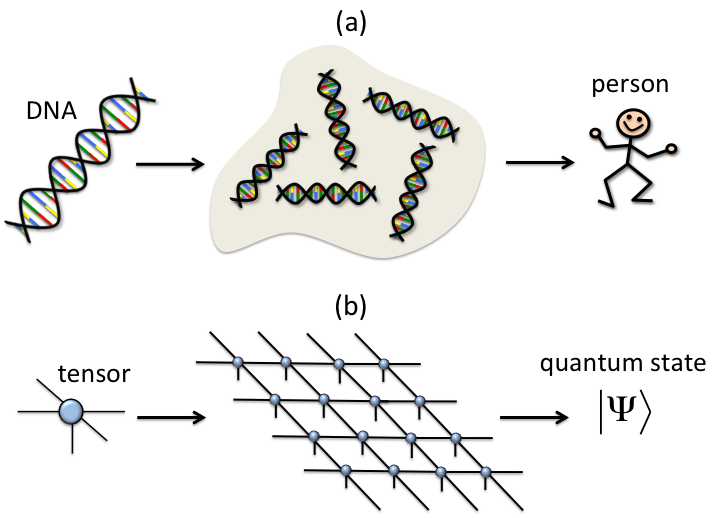
\includegraphics[width=0.99\linewidth]{cartoon.png}
\caption{Example of a figure~\cite{Orus2013}.}
\label{fig:example}
\end{figure}

\bibliography{bibsamp}% Produces the bibliography via BibTeX.


\appendix


\begin{widetext}
\section{Code listing} \label{app:codes}
Please copy your code in the appendix.
\begin{lstlisting}[language=Python]
"""

Module to generate the Hamiltonian of the transverse field Ising model.

H = -J sum_i sigma^x_i sigma^x_{i+1} - g sum_i sigma^z i.

Used in the solution of exercise 5.1

"""

import numpy as np
import scipy
from scipy import sparse
import scipy.sparse.linalg
import matplotlib.pyplot as plt

Id = sparse.csr_matrix(np.eye(2))
Sx = sparse.csr_matrix([[0., 1.], [1., 0.]])
Sz = sparse.csr_matrix([[1., 0.], [0., -1.]])
Splus = sparse.csr_matrix([[0., 1.], [0., 0.]])
Sminus = sparse.csr_matrix([[0., 0.], [1., 0.]])


def singesite_to_full(op, i, L):
    op_list = [Id]*L  # = [Id, Id, Id ...] with L entries
    op_list[i] = op
    full = op_list[0]
    for op_i in op_list[1:]:
        full = sparse.kron(full, op_i, format="csr")
    return full


def gen_sx_list(L):
    return [singesite_to_full(Sx, i, L) for i in range(L)]


def gen_sz_list(L):
    return [singesite_to_full(Sz, i, L) for i in range(L)]


def gen_hamiltonian_periodic(sx_list, sz_list, g, J=1.):
    """ assumes periodic boundery conditions """
    L = len(sx_list)
    H = sparse.csr_matrix((2**L, 2**L))
    for j in range(L):
        H = H - J *( sx_list[j] * sx_list[(j+1)%L])
        H = H - g * sz_list[j]
    return H
\end{lstlisting}
\end{widetext}

\title{Machine Learning of Many Body Localization}

\author{Philipp Krüger}

\date{\today}% It is always \today, today,
             %  but any date may be explicitly specified

\begin{abstract}
Exact diagonalization was used to find the reduced density matrices of the lowest energy eigenstate of the Heisenberg Model with an additional field in z-direction at low and high disorder strength. The resulting dataset representing extended and localized phases, was used to train a neural network to deduct the critical disorder strength for a phase transition. 
%todo About 5% of article length & < 500 words
\end{abstract}


\maketitle

\section{Introduction}%todo: Action title

Review Literature on task

Why is the topic interesting? => Finding Wc?

\subsection{Hamiltonian of the Heisenberg model}

What is it used for? With $J=1$, $h_i \in \left[-W, W\right]$

\begin{equation}
	H=\underbrace{J\sum_i \vec{S}_i\cdot\vec{S}_{i+1}}_{\text{Exchange Energy}}-\underbrace{\sum_ih_iS_i^z}_{\text{Random Field}}
\end{equation}

Outcome expectation: 

In the ergodic phase (delocalized phase) $h<h_c$, the many-body eigenstates
are thermal,20–23 so the isolated quantum system can relax to
thermal equilibrium under the dynamics due to its Hamiltonian.
In the thermodynamic limit $L\rightarrow\infty$, the system thus
successfully serves as its own heat bath in the ergodic phase.
In a thermal eigenstate, the reduced density operator of a
finite subsystem converges to the equilibrium thermal distribution
for $L\rightarrow\infty$. Thus the entanglement entropy between a
finite subsystem and the remainder of the system is, for  $L\rightarrow\infty$, the thermal equilibrium entropy of the subsystem. At
nonzero temperature, this entanglement entropy is extensive,
proportional to the number of degrees of freedom in the subsystem.


In the many-body localized phase $h>h_c$, on the other
hand, the many-body eigenstates are not thermal:2 the
“eigenstate-thermalization hypothesis”20–23 is false in the
localized phase. Thus in the localized phase, the isolated
quantum system does not relax to thermal equilibrium
under the dynamics of its Hamiltonian. The infinite system
fails to be a heat bath that can equilibrate itself. It is a
“glass” whose local configurations at all times are set by the
initial conditions. Here the eigenstates do not have extensive
entanglement, making them accessible to density-matrixrenormalization-group–type
numerical techniques.5 A limit
of the localized phase that is simple is J= 0 with $h>0$. Here
the spins do not interact, all that happens dynamically is
local Larmor precession of the spins about their localrandom
fields. No transport of energy or spin happens and
the many-body eigenstates are simply product states with
each spin either “up” or “down.”
\url{https://doi.org/10.1103/PhysRevB.82.174411}


non-thermalising phase, in which the system violates the Eigenstate Thermalisation hypothesis
\url{https://arxiv.org/pdf/1610.03042.pdf}


J<g: (large W) localized phase (adiabatically connected to trivial state), J>g extended phase (small W) (ordered??)

Is scaling important?

\subsection{Exact Diagonalization}

Introduce concepts: Exact Diagonalization, 

\subsection{Areal (reduced??) Density Matrix}

areal Density Matrix:
\url{http://www.thphys.nuim.ie/staff/jvala/Lecture_9.pdf}

\begin{figure}[h!]
	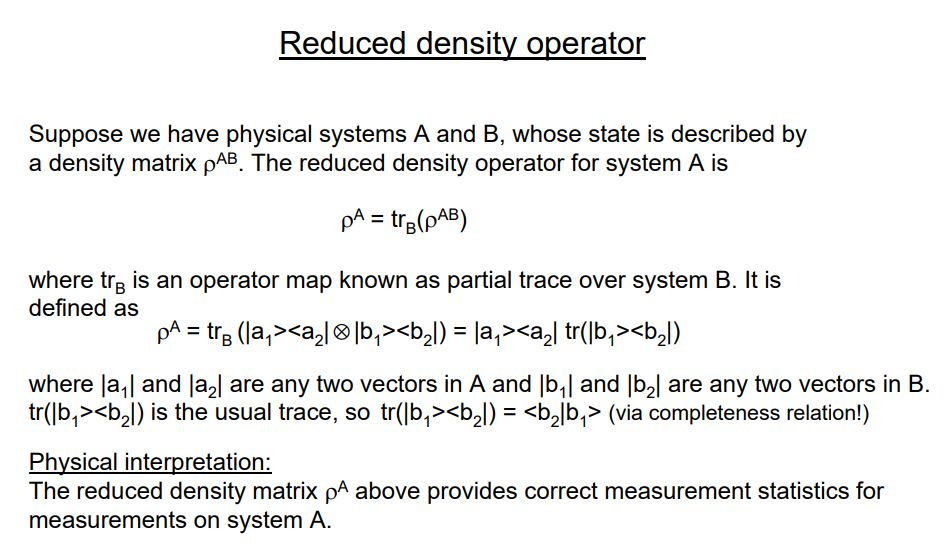
\includegraphics[width=0.99\linewidth]{figures/reduced_density_matrix.jpg}
	\caption{Example of a figure~\cite{Orus2013}.}
	\label{fig:adm}
\end{figure}

vs

direct density matrix:
(DOI: 10.1103/PhysRevB.99.054208 says 
Instead of dividing the system into two subsystems A
and B to calculate the reduced density matrix of an eigenstate rho a and using the entanglement spectrum as the training data set 34,35, we directly feed the
probability density of the eigenstate psi i computed in the
spin basis to the machines as the training data set. The
reason for doing so is that, although by preprocessing
the training data can reduce the dimension and filter out
redundant information, useful information contained in
the wavefunction of the entire system can also be lost.)

Conclusion: => areal

\subsection{Neural Networks and Convolutional Neural Networks}

Neural Network, CNN





\section{Materials and Methods}%todo: Action title

\subsection{Code Protocol}

Explain Flow with figure

\begin{figure}[h!]
	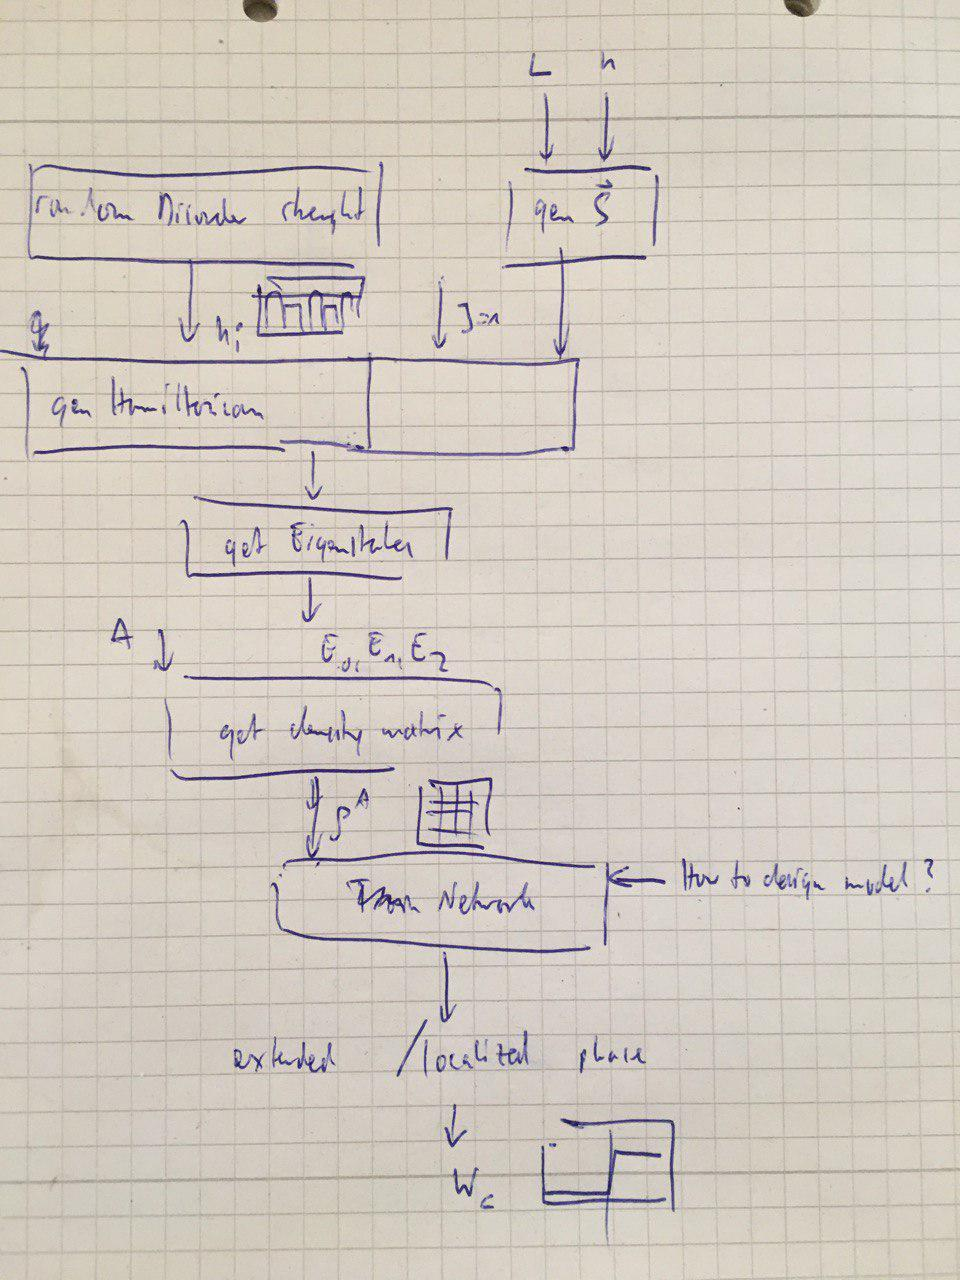
\includegraphics[width=0.99\linewidth]{figures/flowchart.jpg}
	\caption{Example of a figure~\cite{Orus2013}.}
	\label{fig:example}
\end{figure}

Fig.~\ref{fig:example}

\subsection{Machine Learning Models and Error Metrics}

Loss: SparseCategoricalCrossentropy from \url{https://keras.io/api/losses/}

Optimizer: Adam

Explain metrics and errors and why they are used. Which ml models are used and why?

Hyperparameters? Amount of layers?

\section{Results}%todo: Action title

\subsection{Generation of density matrix training set}

Chosen parameters: $L \in \{10, 11, 12\}$. Repetitions: 100. Measure of variation in the test set??

\newpage
\begin{figure}[h!]
	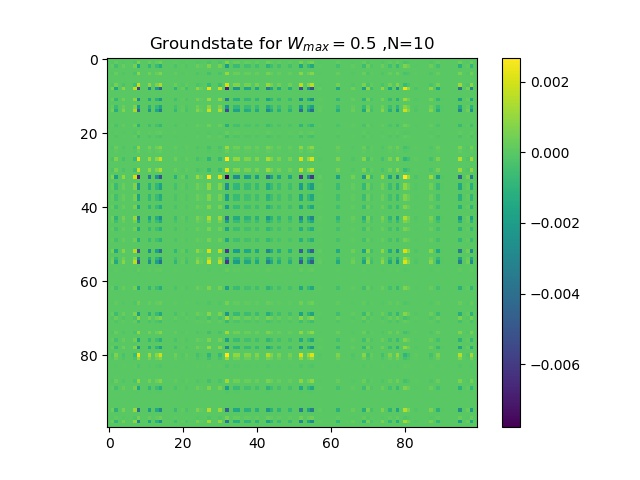
\includegraphics[width=\linewidth]{../results/N10_trainingset_groundstate_Wmax0.5.jpg}
	\caption{Real part of the density matrix of an ergodic phase N = 10.}
\end{figure}
\begin{figure}[h!]
	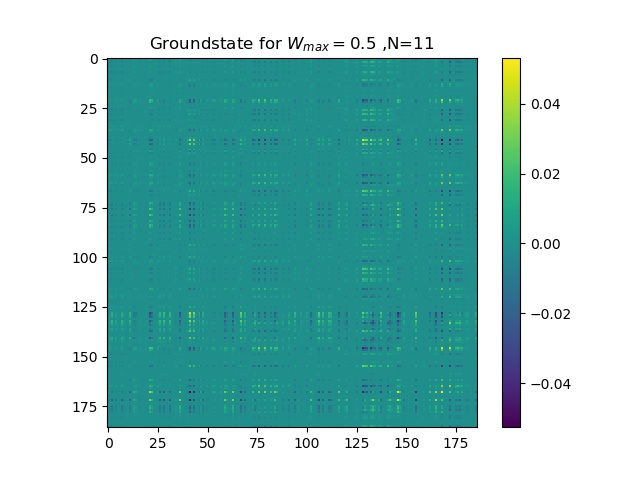
\includegraphics[width=\linewidth]{../results/N11_trainingset_groundstate_Wmax0.5.jpg}
	\caption{Real part of the density matrix of an ergodic phase N = 11.}
\end{figure}
\begin{figure}[h!]
	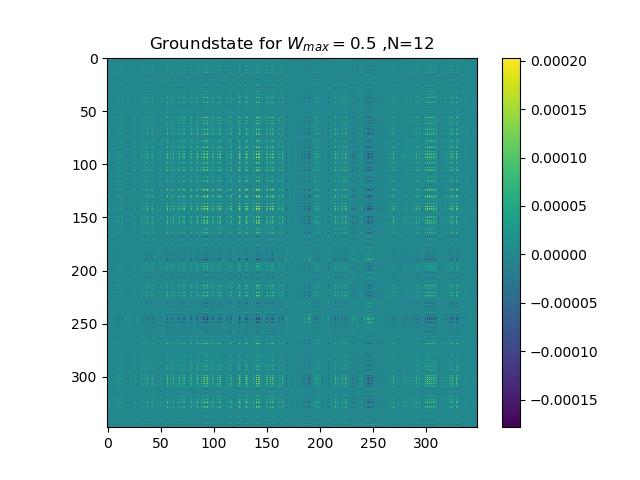
\includegraphics[width=\linewidth]{../results/N12_trainingset_groundstate_Wmax0.5.jpg}
	\caption{Real part of the density matrix of an ergodic phase N = 12.}
\end{figure}
\begin{figure}[h!]
	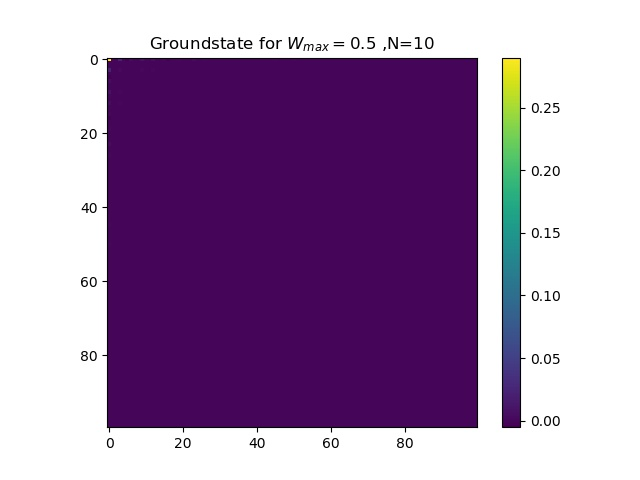
\includegraphics[width=\linewidth]{../results/N10_trainingset_groundstate_Wmax8.0.jpg}
	\caption{Real part of the density matrix of an localized phase N = 10.}
\end{figure}
\begin{figure}[h!]
	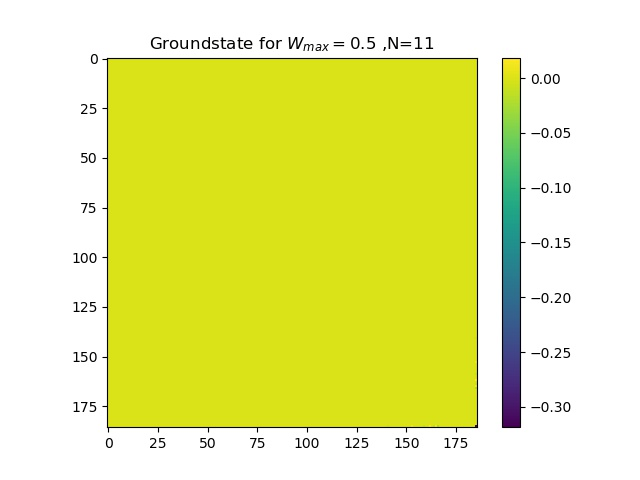
\includegraphics[width=\linewidth]{../results/N11_trainingset_groundstate_Wmax8.0.jpg}
	\caption{Real part of the density matrix of an localized phase N = 11.}
\end{figure}
\begin{figure}[h!]
	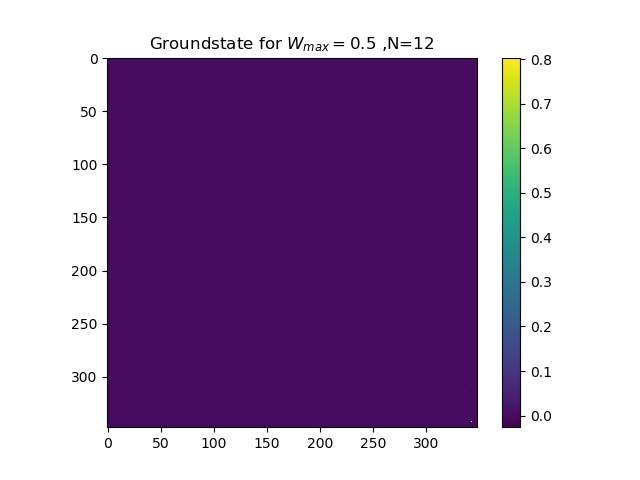
\includegraphics[width=\linewidth]{../results/N12_trainingset_groundstate_Wmax8.0.jpg}
	\caption{Real part of the density matrix of an localized phase N = 12.}
\end{figure}

%\begin{figure}
%	\begin{subfigure}[c]{0.2\textwidth}
%			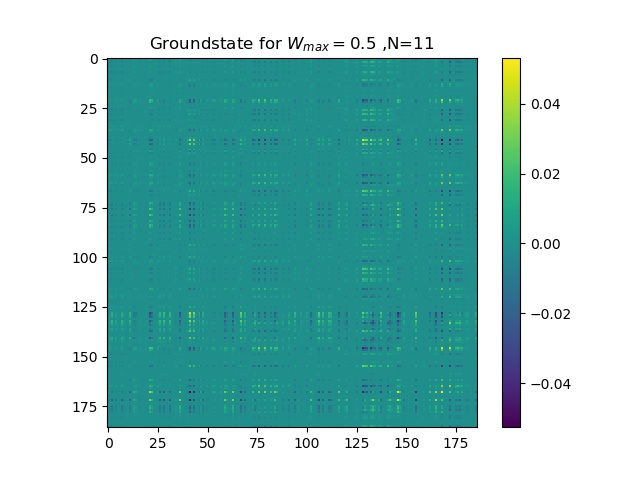
\includegraphics[width=\textwidth]{../results/N11_trainingset_groundstate_Wmax0.5.jpg}
%		\subcaption{}
%	\end{subfigure}
%	\begin{subfigure}[c]{0.2\textwidth}
%		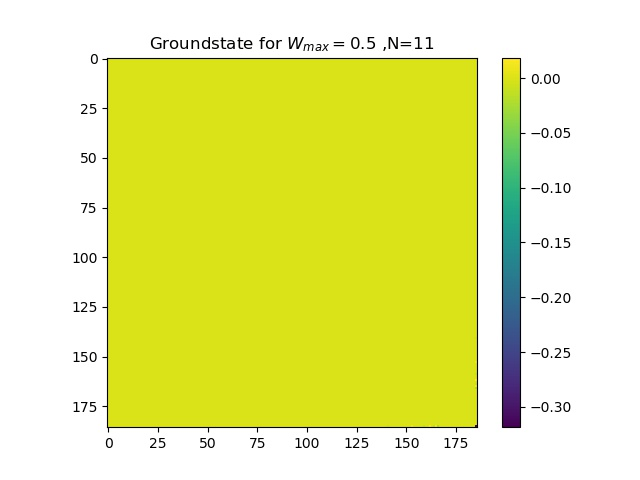
\includegraphics[width=\textwidth]{../results/N11_trainingset_groundstate_Wmax8.0.jpg}
%		\subcaption{}
%	\end{subfigure}
%	\caption{Zwei Bilder mit Subfigure nebeneinander}
%\end{figure}


Plots: 
What is computationally realizable in 1h concerning time?
The training set was sufficiently large enough 

We only need M Eigenstates

This is how corresponding density matrices look like

This will be our parameter space for n, L

\subsection{Prediction of extended vs localized phase}

Training and validation scores:

\begin{figure}[h!]
\centering
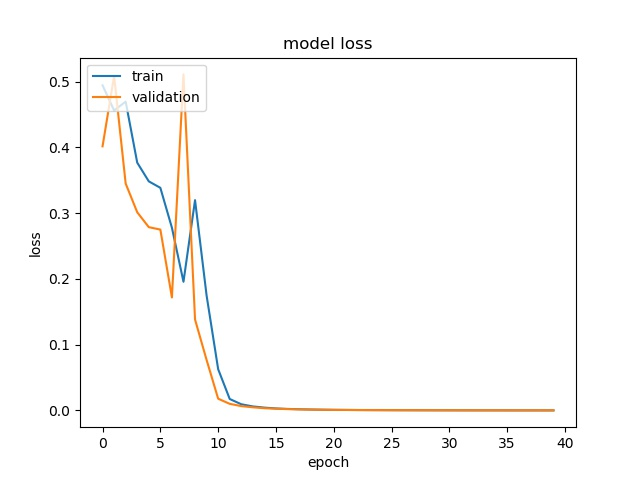
\includegraphics[width=0.7\linewidth]{../results/N10_loss_epochs}
\caption{}
\label{fig:N10_loss_epochs}
\end{figure}
\begin{figure}[h!]
	\centering
	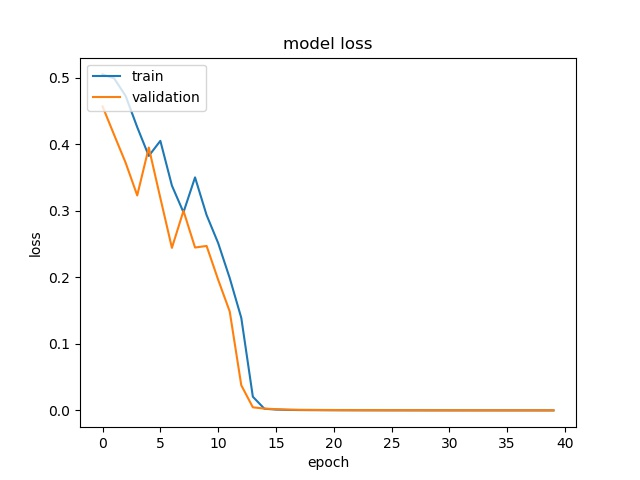
\includegraphics[width=0.7\linewidth]{../results/N11_loss_epochs}
	\caption{}
	\label{fig:N11_loss_epochs}
\end{figure}
\begin{figure}[h!]
	\centering
	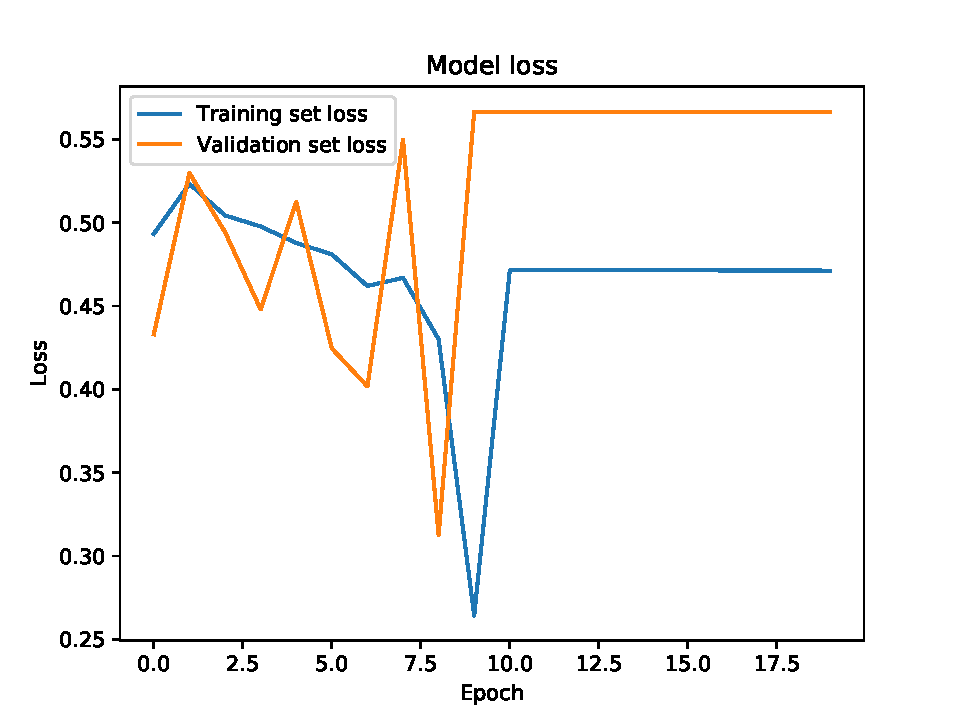
\includegraphics[width=0.7\linewidth]{../results/N12_loss_epochs}
	\caption{}
	\label{fig:N12_loss_epochs}
\end{figure}

\subsection{$W_c$ analysis}


Now we generate testing set with $W_{max} \in \left[0,4\right]$. We suspect $W_c$ to be at 1 ??%todo
We fit a logistic curve and extract $W_c$ as a parameter.

\begin{figure}[h!]
	\centering
	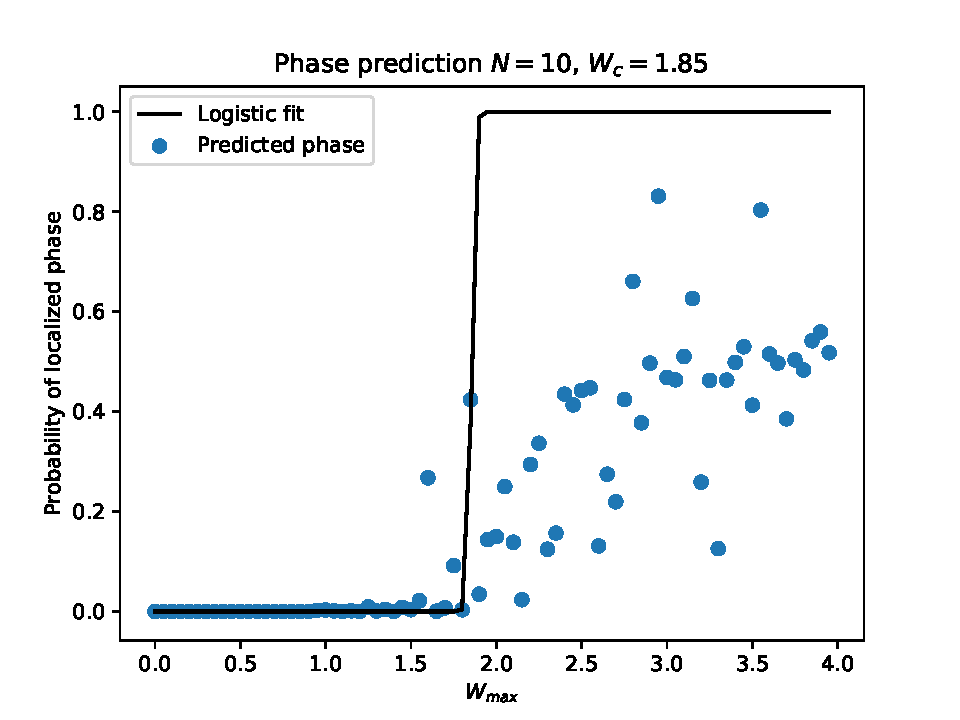
\includegraphics[width=0.7\linewidth]{../results/N10_predict_wc}
	\caption{}
	\label{fig:N10_predict_wc}
\end{figure}

\begin{figure}[h!]
	\centering
	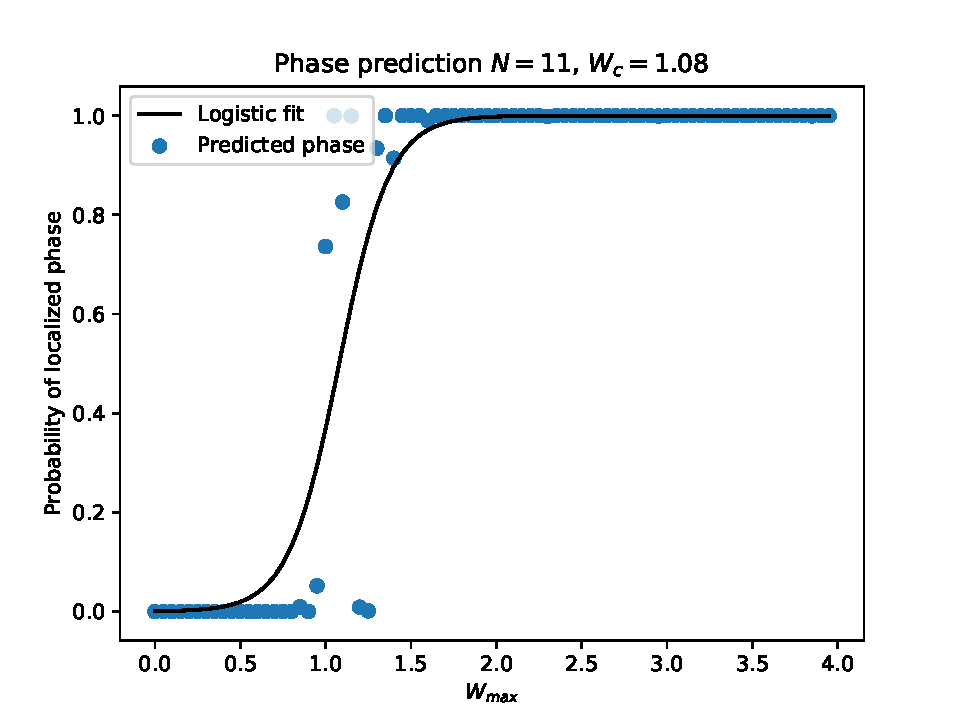
\includegraphics[width=0.7\linewidth]{../results/N11_predict_wc}
	\caption{}
	\label{fig:N11_predict_wc}
\end{figure}

\begin{figure}[h!]
	\centering
	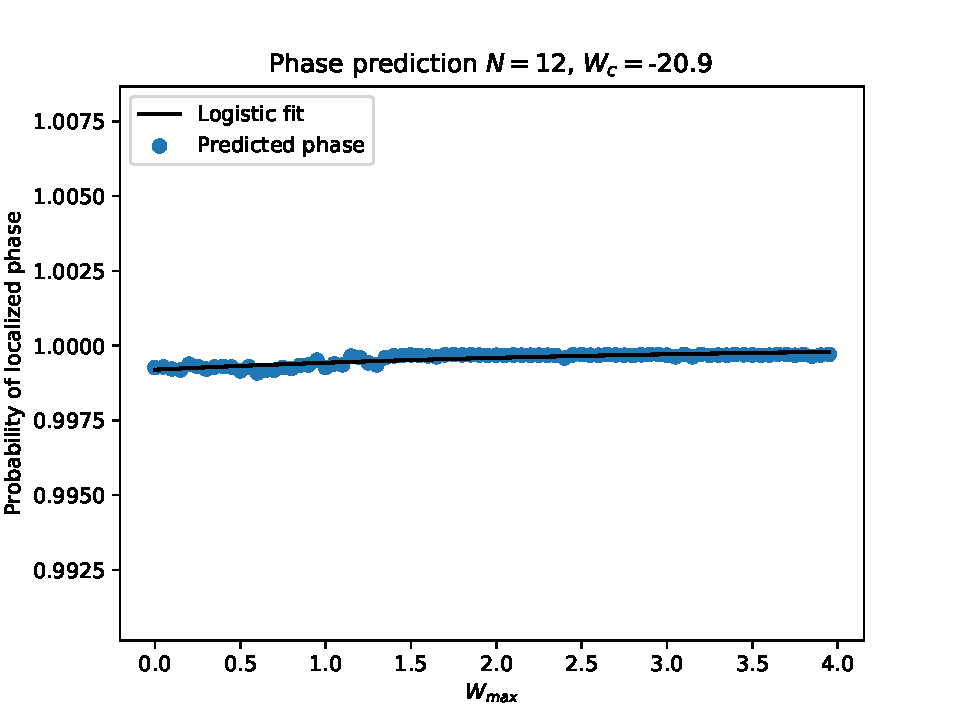
\includegraphics[width=0.7\linewidth]{../results/N12_predict_wc}
	\caption{}
	\label{fig:N12_predict_wc}
\end{figure}


These are our $W_c$ depending on n, L.

%todo: Plot with extracted $W_Cs$

\begin{figure}
	\centering
	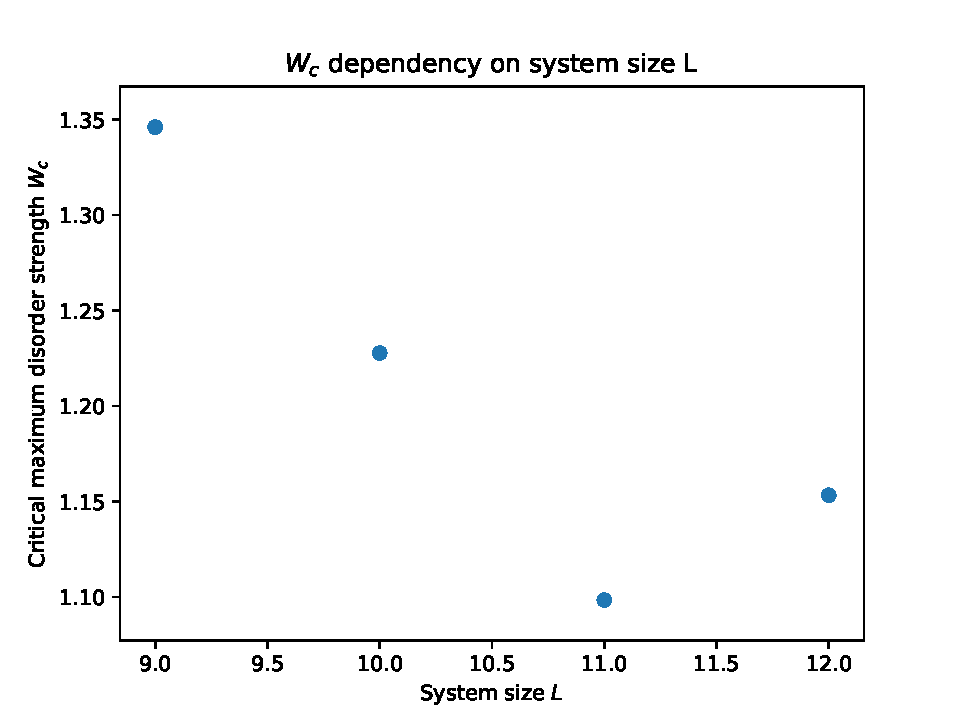
\includegraphics[width=0.7\linewidth]{../results/Wc_L_dependency}
	\caption{}
	\label{fig:Wc_L_dependency}
\end{figure}
\begin{figure}
\centering
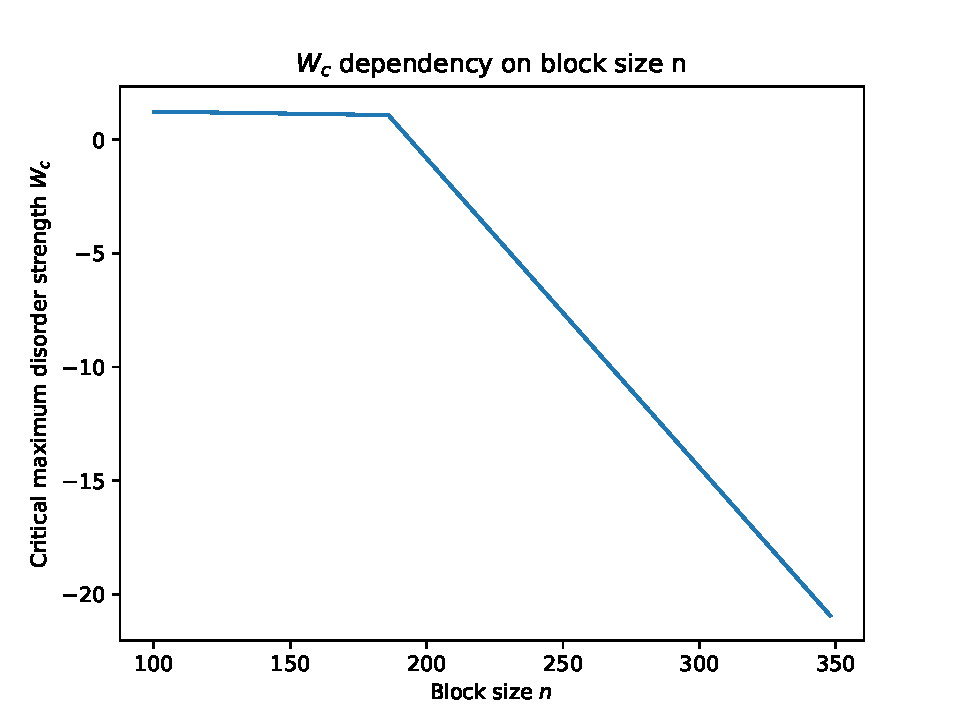
\includegraphics[width=0.7\linewidth]{../results/Wc_N_dependency}
\caption{}
\label{fig:Wc_N_dependency}
\end{figure}


\section{Conclusion}%todo: Action title

$W_c$ depends on n, L (yes/no).

$W_c$ prediction coincides with the expectation (yes/no)

$W_c$ is dependent on these and that effects => scaling analysis? (yes/no)

Citations are numerical\cite{epr}, some more citations~\cite{feyn54,Bire82,Berman1983,witten2001,Davies1998}. 


\bibliography{bibsamp}% Produces the bibliography via BibTeX.


\appendix


\begin{widetext}
\section{Code listing} \label{app:codes}
Please copy your code in the appendix.
\begin{lstlisting}[language=Python]
"""

Description

"""

import numpy as np

code
\end{lstlisting}
\end{widetext}



\end{document}
